% Aharonov-Bohm set-up: two paths around a shielded solenoid; F = 0 wherever the electron goes.
\documentclass[tikz,border=4pt]{standalone}
\usepackage{amsmath,amssymb}
\usetikzlibrary{arrows.meta,decorations.markings,patterns}
\definecolor{p1}{HTML}{2F6DB5}\definecolor{p2}{HTML}{2E9E6B}\definecolor{bcol}{HTML}{D1552B}
\begin{document}
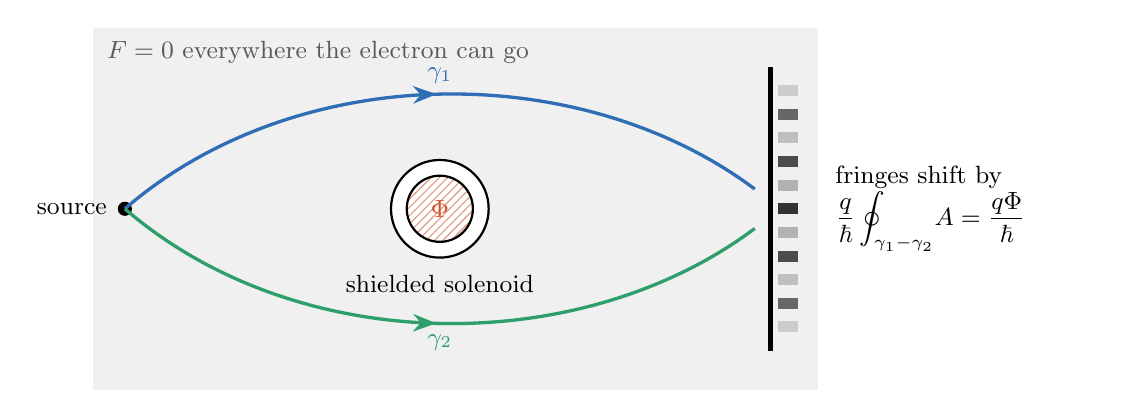
\begin{tikzpicture}[>=Stealth, every node/.style={font=\small}]
\fill[gray!12] (-0.4,-2.3) rectangle (8.8,2.3);
\node[gray!70!black, anchor=north west] at (-0.35,2.25) {$F = 0$ everywhere the electron can go};
% source
\fill (0,0) circle (0.09) node[left=3pt] {source};
% solenoid
\fill[white] (4,0) circle (0.62);
\draw[thick, pattern=north east lines, pattern color=bcol!60] (4,0) circle (0.42);
\draw[thick] (4,0) circle (0.62);
\node[bcol] at (4,0) {$\Phi$};
\node at (4,-0.95) {shielded solenoid};
% paths
\draw[p1, very thick, postaction={decorate}, decoration={markings, mark=at position 0.5 with {\arrow{>}}}]
  (0,0) .. controls (2.2,1.9) and (5.8,1.9) .. (8,0.25) node[midway, above] {$\gamma_1$};
\draw[p2, very thick, postaction={decorate}, decoration={markings, mark=at position 0.5 with {\arrow{>}}}]
  (0,0) .. controls (2.2,-1.9) and (5.8,-1.9) .. (8,-0.25) node[midway, below] {$\gamma_2$};
% screen
\draw[ultra thick] (8.2,-1.8) -- (8.2,1.8);
\foreach \y/\o in {-1.5/20,-1.2/60,-0.9/25,-0.6/70,-0.3/30,0/80,0.3/30,0.6/70,0.9/25,1.2/60,1.5/20}
  \fill[black!\o] (8.3,\y-0.07) rectangle (8.55,\y+0.07);
\node[anchor=west] at (8.9,0) {\parbox{3.3cm}{fringes shift by\\ $\dfrac{q}{\hbar}\displaystyle\oint_{\gamma_1-\gamma_2}\! A = \dfrac{q\Phi}{\hbar}$}};
\end{tikzpicture}
\end{document}
